\thispagestyle{myheadings} % should I be including this at the top of every section page??

\graphicspath{ {Body/Figures/ExperimentalOverview/Decay/} {Body/Figures/TrackingFigures/TrackerPics/} {Body/Figures/ExperimentalOverview/Ring/} {Body/Figures/ExperimentalOverview/Auxiliary/}}

\chapter{Muon g-2 at Fermilab, E989}
\label{chapter:Muon g-2 at Fermilab, E989}

\section{Principle Technique}
\label{sec:PrincipleTechnique}

In a dipole magnetic field, particles will orbit at the cyclotron frequency 
        \begin{align} \label{eq:wc}
        	\omega_{c} = -\frac{Qe}{\gamma m}B,
        \end{align}
and their spins will turn at the precession frequency
        \begin{align} \label{eq:ws}
        	\omega_{s} = -g\frac{Qe}{2m}B - (1-\gamma)\frac{Qe}{\gamma m}B,
        \end{align}
where $Q = \pm 1$ and $e > 0$. The difference between these two frequencies gives
        \begin{align} \label{eq:wasimple}
        	\omega_{a} = \omega_{s} - \omega_{c} = -\frac{g-2}{2}\frac{Qe}{m}B = - a \frac{Qe}{m}B,
        \end{align}
a measureable frequency that is directly proportional to the property of significance, the anamoly a. By measuring the spin difference frequency for muons and the magnetic field B, \amu can be determined. In the presence of an electric field, which is useful in storing the muon beam within a dipole magnetic field, this expands to 
        \begin{align} \label{eq:waelectric}
            \vec{\omega}_{a} = -\frac{Qe}{m} [a_{\mu}\vec{B} - (a_{\mu} - \frac{1}{\gamma^{2}-1})(\vec{\beta} \times \vec{E}) ],
        \end{align}
where now the measurable quanties are vector quantities. Finally, for realistic cases of muon momentum which is non-orthogonal to the magnetic field, the spin difference frequency becomes
        \begin{align} \label{eq:wafinal}
            \vec{\omega}_{a} = -\frac{Qe}{m} [a_{\mu}\vec{B} - a_{\mu} (\frac{\gamma}{\gamma+1})(\vec{\beta} \cdot \vec{B})\vec{B} - (a_{\mu} - \frac{1}{\gamma^{2}-1})(\vec{\beta} \times \vec{E}) ].
        \end{align}
If the motion of the muons is largely perpendicular to the magnetic field, then the second term is small and can be corrected for. If the particles have a momentum of approximately 3.09 GeV/c, the so called ``magic momentum,'' then the third term is small and can be corrected for. These will be talked about later.

In order to measure the spin difference frequency of the muon, a clever technique is used. Decay muons in the pion rest frame are 100\% polarized due to conservation of angular momentum and the fact that the decay neutrino must have a specific helicity. Within a pion beam then the highest and lowest energy decay muons are polarized. Muons will 
decay to positrons with a lifetime of about 2.2 $\mu$s, and the positrons with the highest energies will be correlated with the muon spin, a so called ``self-analyzing'' decay. The single available decay state for a maximum energy positron illustrates this in Figure \ref{fig:MuonDecay}. Thus, by aquiring a large sample of polarized muons and injecting them into a storage ring 

\begin{figure}[]
	\centering
	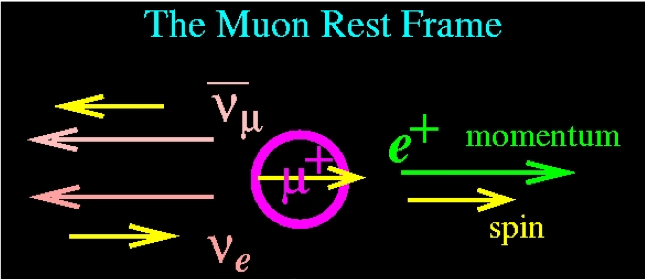
\includegraphics[width=0.9\textwidth]{MuonDecay}
    \caption[Muon Decay - Max Energy Positron]{Make a new version of this picture, and improve this caption.: The single available decay state for maximum energy decay positrons. Due to the conservation of angular momentum and the single possible helicity states of the decay neutrino and anti-neutrino, the spin of the decay positron is exactly equal to the spin of the muon at the time of the decay.}
    \label{fig:MuonDecay}
\end{figure}



-explain the physics
-explain how we get at the physics with our ring and detectors
-parity violation
-actually write out the decay states before explaining some things - well shouldn't these have been talked about before?? maybe not
-decay probabilities and all that
-don't measure all decay positrons
-By injecting a large ensemble of muons and 
-by measuring a subset of ensemble of muons....
-Careful with spin vs polarization





\begin{figure}[]
    \centering
    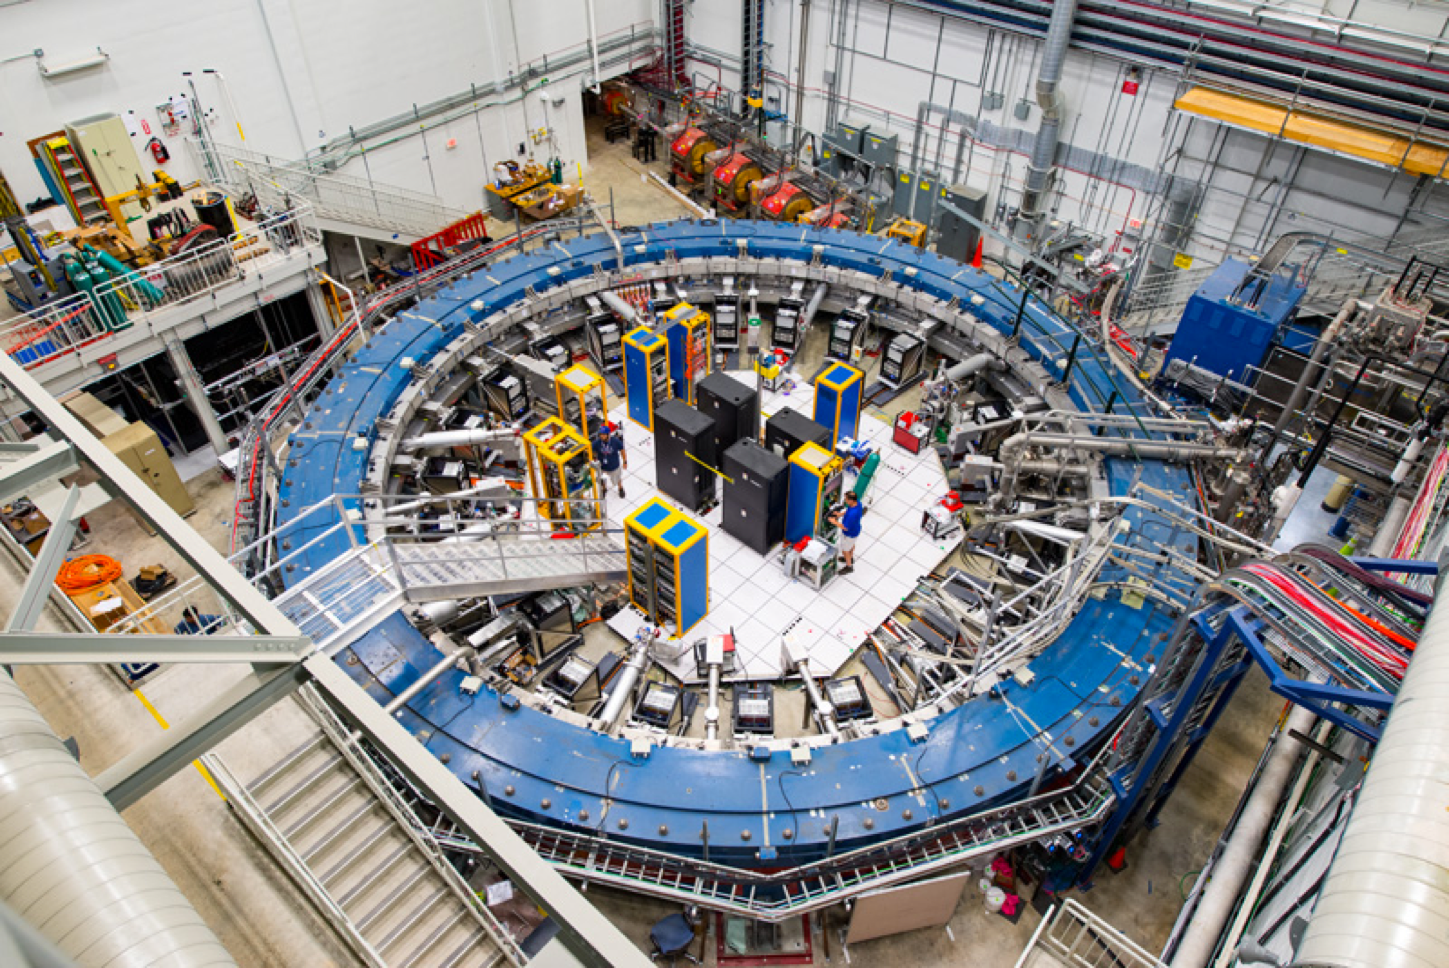
\includegraphics[width=0.9\textwidth]{ring}
    \caption[ring]{clean up and possibly replace}   
    \label{fig:ring}
\end{figure}


\section{Accelerator}
\label{sec:Accelerator}


\cite{Stratakis:2017uci}


\section{Detector Systems}
\label{sec:DetectorSystems}

-how should I order these sections? perhaps by what the beam sees in order?

\subsection{T0}
\label{sec:T0}

In order to align the decay positron spectra in time from fill to fill, an entrace ``T0'' detector is used.  It is made up of a scintillating paddle connected to two (2-inch Hammatsu?) PMTs (photo-multiplier tubes), and is placed just on the outside of the ring before the inflector. See Figure \ref{fig:T0}. One of the PMTs serves as the actual T0 counter which provides an average time of the incoming beam with which to align the fills. The second paddle acts as a magnitude counter to serve as a proxy for the fill intensity. Together they provide a measure of the injected beam profile in time. The varying intensity and bunch shapes can be seen as shown in Figure \ref{fig:T0pulses}.

-might use the same WFD as Calo 1...
-cite all this, with the TDR or hopefully something else \cite{TDR} - can possibly just cite DocDBs as well - need to figure that out
-double check all this - just wrote from memory, also add detail - might want to just explain things better too, ``one PMT with low pe stats and one with high pe stats'' and how that works in the way I've already described above - ND (neutral density filters) one at 1\% one at 10\%
-if I use p.e. include it in the abbreviations
-get a picture of a T0 output from the midas page, also possibly comparing various bunches
-docDB 10911 for details
-docDB 10162 for pictures by Hannah


\begin{figure}[]
    \centering
    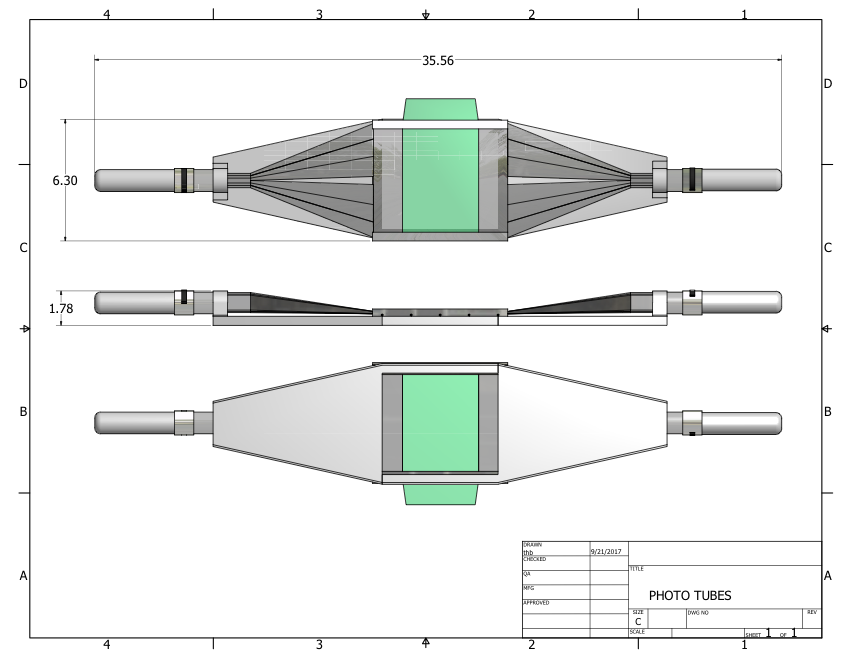
\includegraphics[width=0.9\textwidth]{T0}
    \caption[T0 Counter]{Shown is the T0 entrance counter. In the center in green is the scintillator, which connects with light guides to PMTs on the left and right. Each PMT has a separate ND (what's this?) filter to modify the light output into each PMT to configure one more for fill timing, and the other for fill intensity.}
    \label{fig:T0}
\end{figure}

\begin{figure}[]
    \centering
    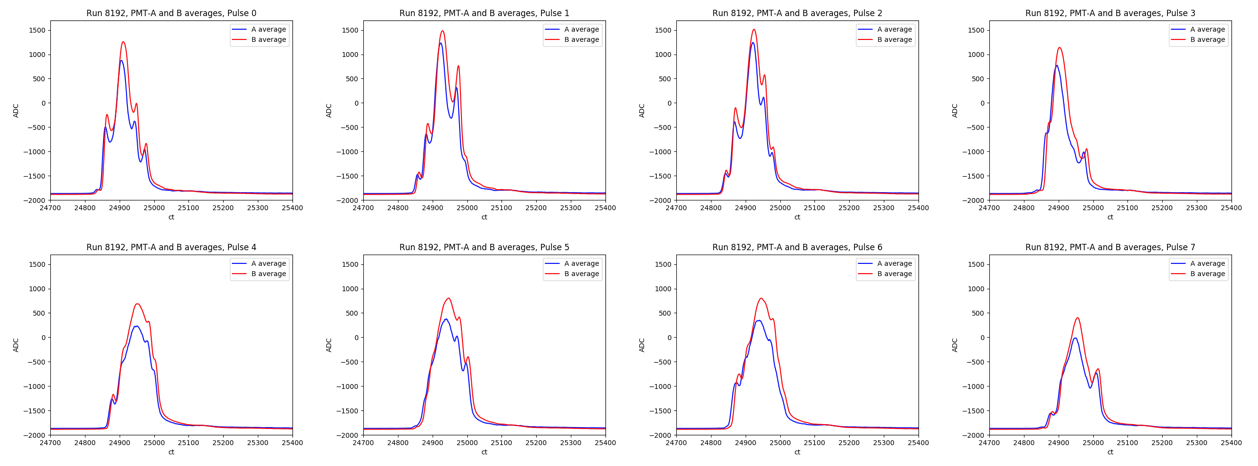
\includegraphics[width=0.9\textwidth]{T0pulses}
    \caption[T0 Pulses]{Shown are time profiles for the two PMTs (A and B) in the T0 counter for the 8 pulses we receive in an accelerator cycle/bunch/what. (careful here - not quite right) Each profile is an average of 100 such profiles. The x axis is in clock ticks (ct), each of which is 1.25 ns. (I will probably explain cts before this somewhere right?) PMT A is the low stats p.e. phototube and PMT B is the high stats p.e. phototube. Picture is too small, might want to rotate or replace it with somthing.}
    \label{fig:T0pulses}
\end{figure}


\subsection{IBMS}
\label{sec:IBMS}

There are two scintillating fiber detectors which monitor the beam as it passes through the inflector, the so-called inflector beam monitoring system (IBMS). See Figure \ref{fig:IMBS1and2}. These devices are placed at the outside of the magnet yoke before injection into the back hole of the magnet, and at the entrance to the inflector. A third device is planned to be at or near the downstream end of the inflector (fix this later on). See Figure \ref{fig:IBMSPlacement}. These devices are used to verify the beam optics tune in the muon injection through the inflector and continuously diagnose beam properties as a handle on systematic problems.

-justification document - DocDB 2722
-DocDB 10944


\begin{figure}[]
    \centering
    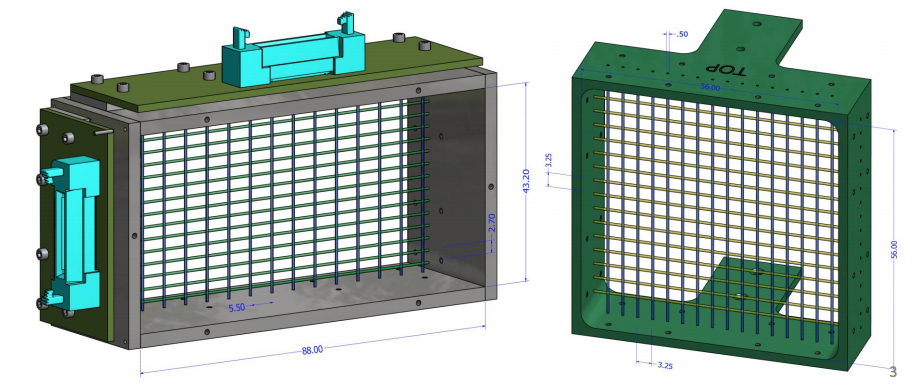
\includegraphics[width=0.9\textwidth]{IBMS1and2}
    \caption[IBMS Models]{Simulation models of the IBMS 1 and 2 detectors. Scintillating fibers form an array which detect particles as they pass through them.}   
    \label{fig:IBMS1and2}
\end{figure}

\begin{figure}[]
    \centering
    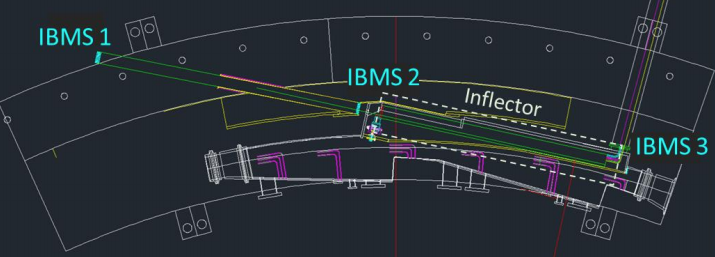
\includegraphics[width=0.9\textwidth]{IBMSPlacement}
    \caption[IBMS Positions]{The positions of IBMS 1, 2, and the planned 3rd system are shown with respect to the vacuum chamber and inflector.}   
    \label{fig:IBMSPlacement}
\end{figure}


\subsection{Fiber Harps}
\label{sec:FiberHarps}

There are four scintillating fiber detectors located within the ring, two at the 180 degree position which measure the vertical and horizontal directions respectively, and similarly at the 270 degree position. One of these devices is shown in Figure \ref{fig:fiberharp}. These `fiber harps' serve to monitor beam properties at all times during a fill, including just after injection and during scraping. This is especially useful as a diagnostic tool as well as a measurement of the central beam position and CBO properties (have I talked about this yet?). Because the fiber harps are a distructive measurement of the beam, they are retractable and are only inserted in special runs in order to make said beam measurements. When they are inserted however they provide a wealth of useful information regarding the beam, as shown in Figure \ref{fig:fiberharp_measurement}.

-DocDB 8366

\begin{figure}[]
    \centering
    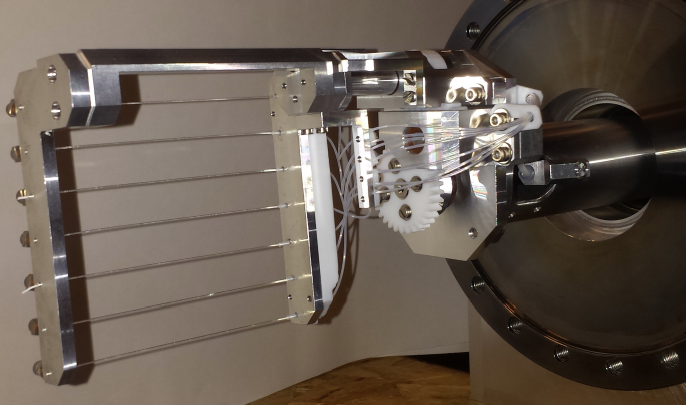
\includegraphics[width=0.9\textwidth]{fiberharp}
    \caption[Fiber Harp]{Picture of one of the fiber harps. A row of 7 scintillating fibers measures the beam instensity as a function of time at various vertical or horizontal components depending on which fiber harp is inserted.}   
    \label{fig:fiberharp}
\end{figure}

\begin{figure}[]
    \centering
    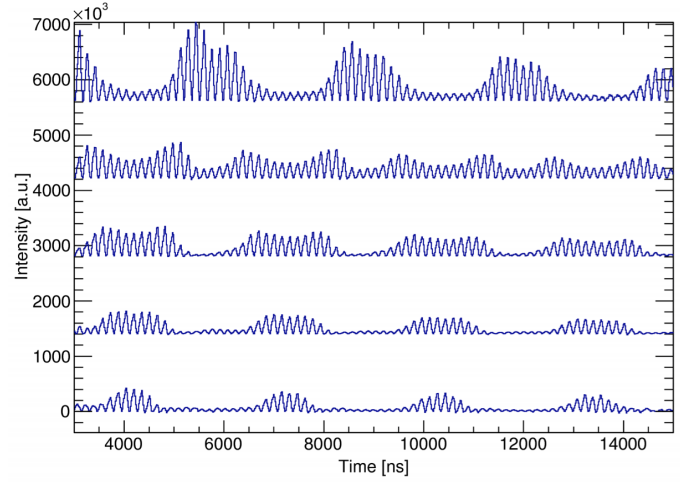
\includegraphics[width=0.9\textwidth]{fiberharp_measurement}
    \caption[Fiber Harp Measurement]{The fiber harps measure beam intensity as a function of time and fiber number. The middle spectrum is the output from the middle fiber, the upper spectra being fibers which are at successively greater radial positions, and the lower spectra being fibers which are at successively lower radial positions. The fast oscillations of the cyclotron frequency can be seen along with the slower oscillations of the CBO. This particular set of data was at a time or run when more beam was on the outside part of the storage region. (This last part is conjecture somewhat - maybe I should leave it out. I might honestly also want to leave out this whole picture, not sure..)}   
    \label{fig:fiberharp_measurement}
\end{figure}




% move this somewhere better
\begin{figure}[]
    \centering
    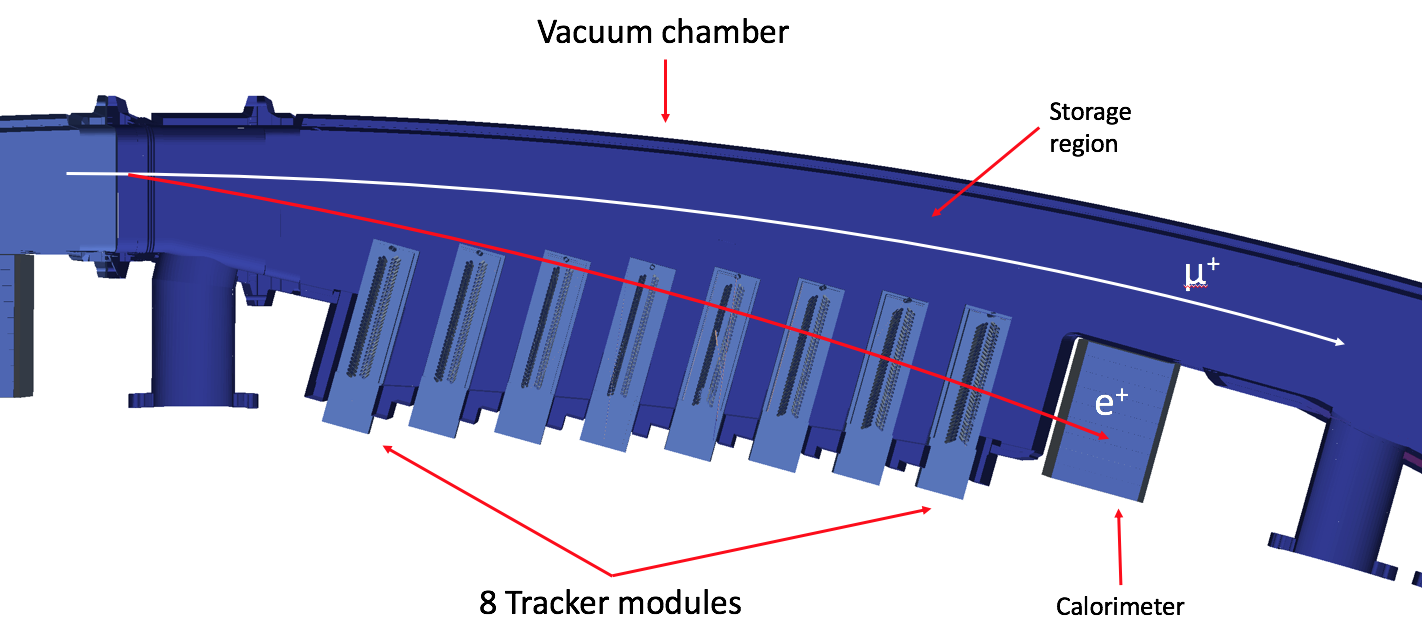
\includegraphics[width=0.9\textwidth]{TrackerCaloWithLines}
    \caption[TrackerCaloWithLines]{Birds eye view of a model of a vacuum chamber containing a tracker station, and the associated calorimeter. Muons pass around the ring in the center of the storage region which is contained within the bulk of the vacuum chamber. The muons decay to positrons, some of which then pass through the trackers or hit calorimeters. Each tracking station consists of 8 tracker modules.}   
    \label{fig:TrackerCaloWithLines}
\end{figure}


\subsection{Calorimeters}
\label{sec:Calorimeters}

% what they do
% what they are
% how they work

Electromagnetic calorimeters measure the times and energies of decay positrons as they curl inward from the storage region. There are 24 calorimeters located symmetrically around the inside of the ring in close proximity to the vacuum chamber, as shown in Figure \ref{fig:TrackerCaloWithLines}. They lie close to the storage region in order to measure a large fraction of the total number of observable decay positrons, including the high energy decay positrons which curl inward only slightly more than the muons themselves do. (max acceptance)

Each calorimeter consists of 54 channels of PbF\textsubscript{2} crystals arrayed in a 6 high by 9 wide array, which measure Cerenkov light emitted by the incident positrons as they pass through the crystals \cite{Fienberg:2014kka}. (Picture of single calo and its crystals here.) Cerenkov light is naturally fast which improves timing resolution of the incoming hits. Each crystal is 2.5 x 2.5 x 14 cm\textsuperscript{3} and is wrapped in black Tedlar\textregistered\ foil to reduce light transmission between crystals and improve position reconstruction, as well as reduce pulse width \cite{Kaspar:2016ofv}. The light is read out by large area silicon photo-multiplier (SiPM) sensors. Each calorimeter sits on a board extending out from a cart containing the electronic which power the calorimeters and read out the data, as shown in Figure \ref{fig:} This is to relocate magnetic material away from the field region to avoid perturbing the field and to remove sensitive electronics from the decay path region. Similarly, due to the close proximity to the storage region and by extension the magnetic field, the calorimeters, the encapsulating material, and the SiPMs are made from non-magnetic material.

In order to determine \amu to the precision goal, there are modest requirements on the performance of the calorimeters. They must have a relative energy resolution of better than 5\% at 2 GeV, in order for proper event selection \cite{TDR}. They must have a timing resolution of better than 100 ps for positrons with greater than 100 MeV energy. The calorimeters must be able to resolve multiple incoming hits through temporal or spatial separation at 100\% efficiency for time separations of greater than 5 ns in order to reduce the pileup systematic error due to the high rate. Finally, the gain of the measured hits must be stable to $<$ 0.1\% over a 200 $\mu$s time period within a fill, and unaffected by a pulse arriving in the same channel a few nanoseconds earlier. The long term gain stability over a time period of order seconds must be $<$ 1\%. The SiPMs chosen satisfy these requirements (as well as the physical ones), due to their fast rise times and consistent pulse shapes. (Should this part be here? Or elsewhere? Before perhaps? Might need to update the gain numbers...)

(I've condensed quite a bit this section from the TDR - is that okay?)

A 12 bit waveform digitizer (WFD) samples each photodetector channel at a rate of 800 MSPS with a 1 Gb memory buffer and the data are transferred to a bank of GPU processors for on-line data processing \cite{Sweigart:2016jty}. The timing resolution of these WFDs is $<$ 50 ps for most pulse amplitudes.

Should I go into the calorimeter DAQ here? Or make that it's own section - how uniform are the DAQ systems for each detector system? Are the same sorts of modules and crates and WFDs used or what? If so it's own section might make sense, otherwise probably include small pieces at the end of each individual detector about the daq system



\subsection{Laser Calibration System}
\label{LaserCalibrationSystem}
% should I make this it's own section? or include at the end of the calo section? probably the latter

In order to satisfy the gain requirements, a laser calibration system was put into place in order to monitor the SiPM responses over short times (fill level), and long term (days to years). By comparing a known signal to the SiPM output. At the front face of each calorimeter is a board containing prisms connected to fibers from the laser system which can be pulsed in-fill or out of fill for each crystal individually. 


-can pulse laser in fill, out of fill, and double pulse
-mention the laser hut at all? probably not


% make sure these are ordered properly - might not need all of them
\cite{Anastasi:2015ssy}
\cite{Anastasi:2016luh}
\cite{Anastasi:2017sos}




\subsection{Straw Trackers}
\label{sec:StrawTrackers}

The Muon \gmtwo Experiment at Fermilab uses straw tracking detectors to measure decay positron trajectories for the purpose of determining the muon beam distribution and its characteristics (and other things....). By fitting these tracks and extrapolating back to the average decay point, the beam can be characterized in a non-destructive fashion. See section blah. This is important because of the need for matching the average observed magnetic field of the decaying muons and their resulting decay positron directions which result in the \wa frequency.

The trackers are also useful for determining general beam diagnostics as well as the pitch correction and to a lesser extent the electric field correction (careful here). Cross-checking separately for pileup removal, hit verification, etc. is a powerful tool. Combining them in order to provide the muon distribution that the calorimeters directly see for the \wa calculation is perhaps the most important role of the tracker. With three trackers, approximately 5\% of decaying muons will result in measureable positron tracks assuming no pileup in the tracker, many of which do not hit the nearest calorimeter.

Each tracker module consists of 4 layers of 32 straws with a stereo angle of 7.5 degrees, the first two ``U'' layers oriented with the tops of the straws at a greater radial position, and the second two ``V'' layers oriented with the bottoms of the straws at a greater radial position. A tracking module is shown in Figure \ref{fig:tracker}. There are 2 tracker stations located in front of calorimeters 13 and 19, or at approximately 180 and 270 degrees counting clockwise from the top most point of the ring where the inflector resides. Figure \ref{fig:WorldCoordSys} shows this. (A third station sits empty after the inflector.) Each station consists of 8 tracking modules arranged in a staircase pattern that follows the curvature of the ring as seen in Figure \ref{fig:staircase}.

\begin{figure}[]
    \centering
    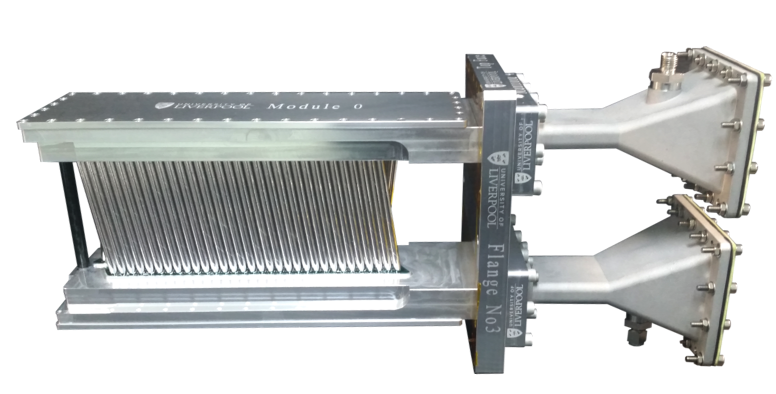
\includegraphics[width=0.9\textwidth]{Tracker}
    \caption[Tracker module]{Shown is a picture of one of the many tracking modules used in the Muon \gmtwo experiment. The first layer of straws with a stereo angle of 7.5 degrees can be seen, with the other 3 straw layers hiding behind it. The beam direction is roughly into the page in this picture, to the left of the end of the module, and this view is what the decay positrons will see.}
    \label{fig:tracker}
\end{figure}

\begin{figure}[]
    \centering
    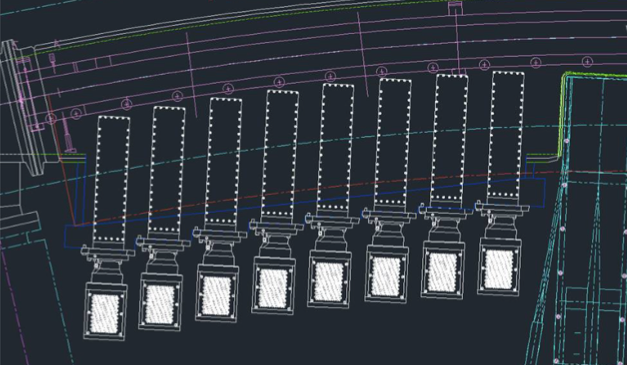
\includegraphics[width=0.9\textwidth]{trackerStation}
    \caption[Tracker module arrangement]{Tracker modules are arranged in the shown staircase pattern. In green and dark blue is the edge of the vacuum chamber (where the dark blue identifies the modification that was made to the old vacuum chambers), and it can be seen that vacuum chamber walls lie at the ends of the outside tracking modules. The position of a calorimeter can be seen in cyan at the right. The dark red spots are the locations of the outside magnet pole tips. From the shown geometry one can see that many positrons will hit either the tracker or the calorimeter but not both due to the acceptance differences.}
    \label{fig:staircase}
\end{figure}

In order to reduce the amount of multiple scattering within the straw tracking chambers as particles pass through them, the material of the straw trackers is minimized. Each straw is made of mylar foil, within which a 25 $\mu$m radius tungsten wire resides, and is filled with Argon-Ethane gas \cite{something}. Fast moving particles ionize the gas as they pass through it, and the resulting ions are drawn to the wire which is held at high voltage. When they reach the wire (and the mylar) a signal can be read out which tells us that a particle was seen to pass through the straw. By combining many such signals in a brief time span, we are able to construct tracks of incidient particles. (See section blah.) The resolution of hits within the straws is approximately 150 $\mu$m \cite{something}.

The signals of the straws are read out through...


